\documentclass[12pt,]{book}
\usepackage[utf8]{inputenc}
\usepackage[T1]{fontenc}
\usepackage{mathptmx}
\usepackage{geometry}
\usepackage{mathtools}
\usepackage[english]{babel}
\usepackage{graphicx}
\usepackage[os=win]{menukeys}
\usepackage[figurename=Gambar]{caption}
\usepackage{hyperref}
\usepackage{minted}

%\addto\captionsenglish{\renewcommand{\contentsname}{Daftar Isi}}

\hypersetup{
	colorlinks=true, %set true if you want colored links
	linktoc=all,     %set to all if you want both sections and subsections linked
	linkcolor=blue,  %choose some color if you want links to stand out
}

\geometry{
	a4paper,
	left=15mm,
	right=10mm,
	top=10mm,
	bottom=10mm,
}

\title{\Large \bf
	Technical Document (Preliminary Design)
}

\author{Achmadi ST s.MT}
\date{}

\begin{document}
	
	\maketitle
	\thispagestyle{empty}
	\pagestyle{empty}
	
	\newpage
	\tableofcontents
	
	\newpage
	\chapter{Joinwit}

	\section{Introduction}
	
	\hspace{10pt} This document explain essential part of development.
	In this development chapter, currently use Joinwit product (as is, no deep reverse engineer).
	All development files (including source of this document) available as open-sources at \url{https://github.com/mekatronik-achmadi/fo_respiro}
	
	The main hardware part section of development consist:
	\begin{itemize}
		\item Optical Power Meter module. Taken from product JW-3208
		\item Laser Source module. Taken from product JW-3109
		\item Custom Central Processor Unit. Using development board Cz-mini STM32F103Vx. Essenstial module consist:
		\begin{itemize}
			\item STM32F103Vx chip, an 32-bit armhf core chip
			\item LCD-TFT based on ILI9320 protocol  
		\end{itemize}
		\item Bluetooth Serial module HC-05
		\item 5v Power Source. Currently using a common powerbank 	
	\end{itemize}

	The main Software part section of development consist:
	\begin{itemize}
		\item a real-time multithreaded firmware based on ChibiOS/RT using both kernel scheduling and hardware abstraction layer.
		\item a desktop interface that data with interchange Custom CPU based Qt5 SDK
		\item a mobile apps interface that data with interchange Custom CPU based on Android SDK
	\end{itemize}

	\section{Hardware}
	
	\subsection{Optical Power Meter}
	This module is used to aquire any raw photonic signal or power.
	This module has no any modification or engineering, except geting ADC input signal that has voltage level compatible with STM32 series chip (custom CPU chip).
	Type and brand used is JW (Joinwit) 3208 series.
	
	\subsection{Laser Source}
	This module is used to provide laser signal/power. 
	This module has no any modification or engineering.
	Type and brand used is JW (Joinwit) 3109 series.
	
	\begin{figure}[h]
		\centering
		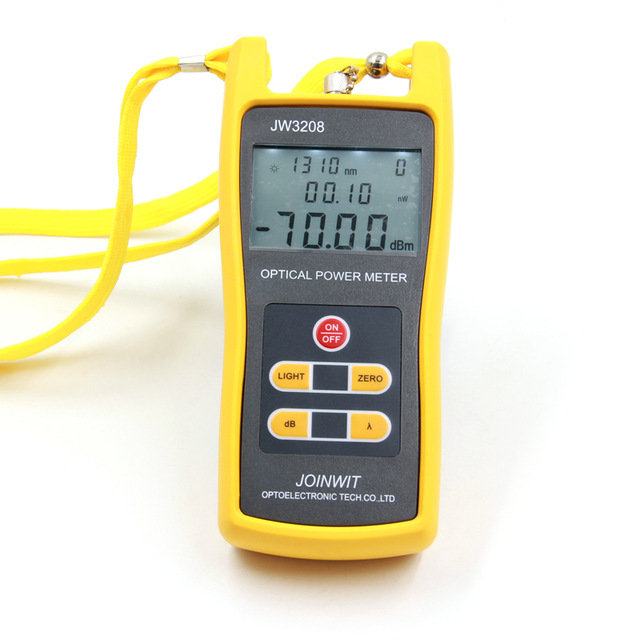
\includegraphics[width=200pt]{images/jw3208}
		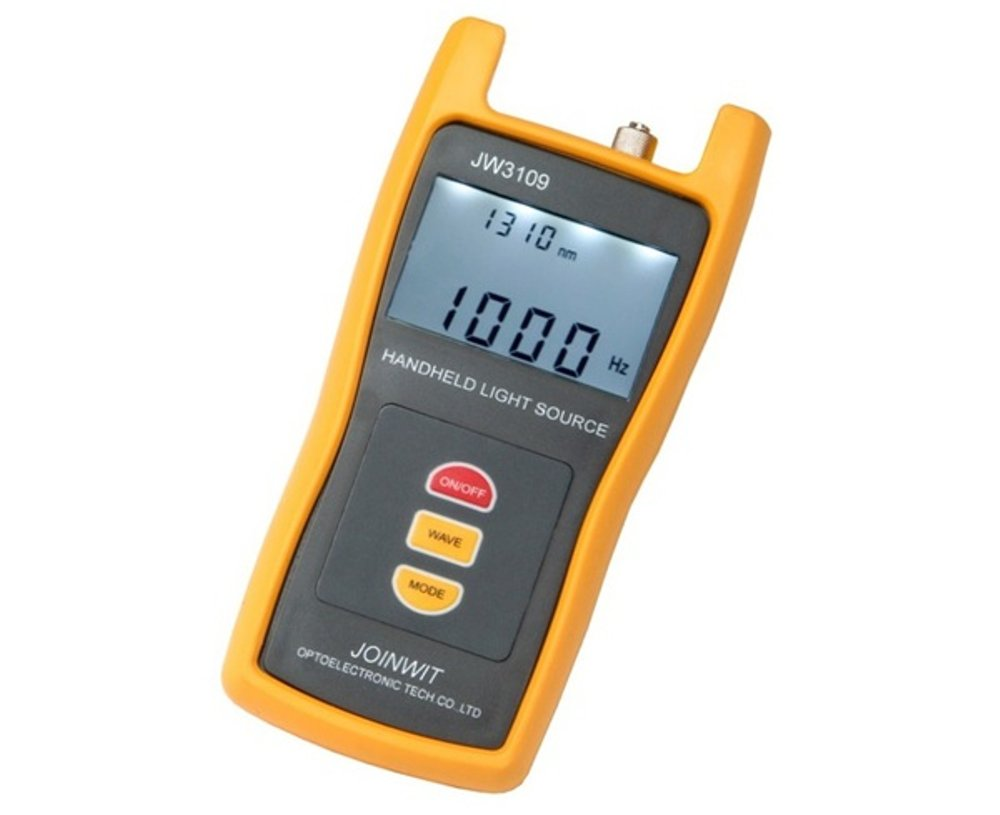
\includegraphics[width=200pt]{images/jw3109}
		\caption{Instrumen JW3208 dan JW3109}
	\end{figure}
	
	\subsection{Custom Central Processing Unit}
	This module (development board )is used as central processing system.
	Type and brand used is CZ-miniSTM32F103Vx.
	
	Internal module used are consist:
	\begin{itemize}
		\item Analog to Digital Converter (ADC) with 12-bit data size to aquire input signal from Optical Power Meter.
		\item Serial data UART (both USB and HC-05) with 8-bit data size to communicate with outside of the chip.
		\item General digital I/O to control Laser Source module.
	\end{itemize}

	\begin{figure}[h]
		\centering
		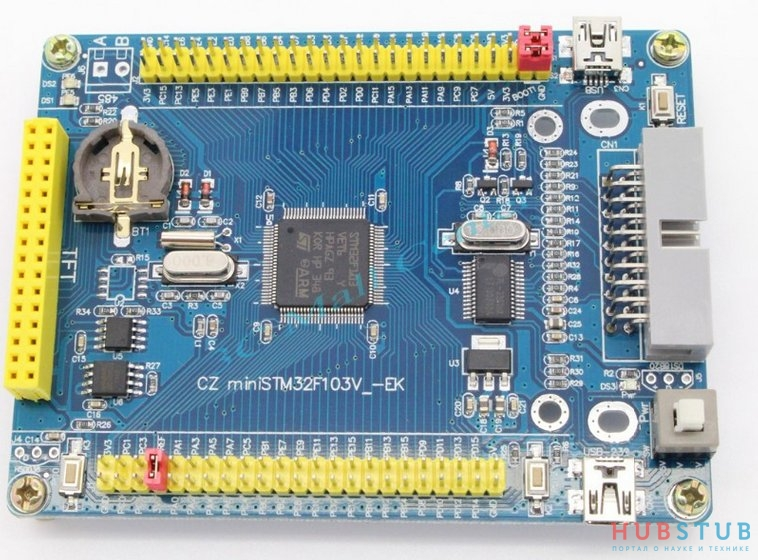
\includegraphics[width=400pt]{images/ministm32f103}
		\caption{Development Board CZ miniSTM32F103Vx}
	\end{figure}

	\newpage
	\subsection{Bluetooth Serial}
	This module is used to provide communication feature with any device (either computer or mobile) that support Bluetooth radio communication. 
	Type and brand used is HC-05.
	
	\begin{figure}[h]
		\centering
		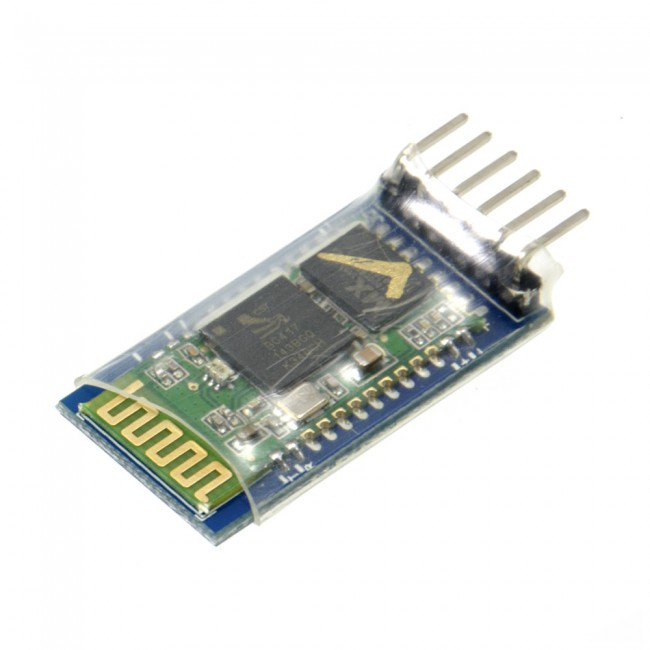
\includegraphics[width=200pt]{images/hc-05}
		\caption{Module Bluetooth HC-05}
	\end{figure}
	
	
	\section{Hardware Bill of Material}
	
	Below are part list for purchasing purposes:
	\begin{itemize}
		\item Optical Power Meter JW-3208 from e-Bay: \url{https://www.ebay.com/p/Joinwit-Handheld-Optical-Power-Meter-JW3208/2191151148}
		\item Laser Source JW-3109 from e-Bay: \url{https://www.ebay.com/p/Jw3109-Handheld-Optical-Light-Source-FC-CONNETCTOR-Fiber-Optic-Tester1310-1550nm/1683352799}
		\item Development Board CZ-MiniSTM32F103Vx from Aliexpress: \url{http://www.aliexpress.com/item/FREE-SHIPPING-ARM-Cortex-M3-mini-stm32-stm32F103VEt6-Cortex-development-board-72MHz-512KFlash-64KRAM/32216480157.html}
		\item LCD-TFT ILI9320 from Aliexpress: \url{https://www.aliexpress.com/item/3-2-inch-37PIN-TFT-LCD-Screen-ILI9320-Drive-IC-240-RGB-320-No-Touch-Panel/32579843844.html}
		\item HC-05 Bluetooth RFComm module from Digiware: \url{http://digiwarestore.com/en/bluetooth/hc-05-bluetooth-module-432241.html}
	\end{itemize}	  
	
	\section{Software}
	
	\subsection{ChibiOS/RT}
	ChibiOS/RT is framework to build high quality firmware for many embedded system chips.
	In this work, both kernel and hardware abstraction are used.
	
	ChibiOS/RT Kernel is the high performance RTOS part of the ChibiOS embedded collection.
	Kernel RT has been designed with the idea of creating a very feature-complete RTOS that could excel in performance and code size.
	
	\begin{figure}[h]
		\centering
		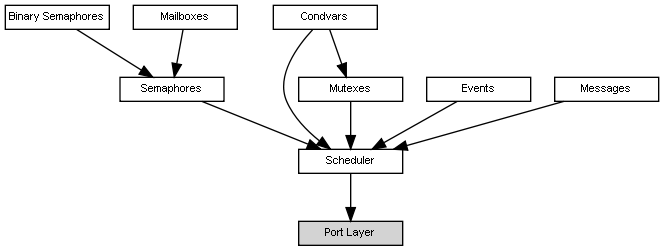
\includegraphics[width=300pt]{images/chibios_kernel}
		\caption{ChibiOS Multithreading Kernel}
	\end{figure}
	
	\newpage
	The HAL component is meant to be an abstraction layer between the application and the underlying micro-controller hardware.
	HAL offers an high level API for accessing common MCU peripheral like GPIO, ADC, SPI and so on and also take care of clocks-related and board-level initializations.
	
	\begin{figure}[h]
		\centering
		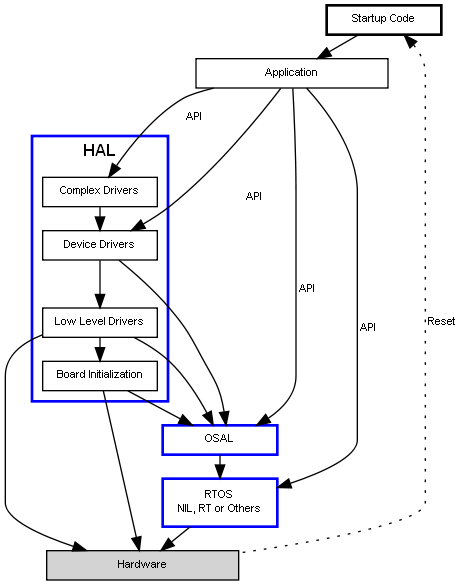
\includegraphics[width=175pt]{images/chibios_hal_arch}
		\caption{ChibiOS Hardware Abstraction Layer}
	\end{figure}

	The main section of firmware consist:
	\begin{itemize}
		\item Analog to Digital COnverter (ADC)
		\item Serial Shell Interface (both for Bluetooth and USB)
		\item Data Handling (include calibration)
		\item LCD-GUI display (both graph and console)		
	\end{itemize}

	By including ChibiOS API, all module dependecies can be described below:
	\begin{figure}[h]
		\centering
		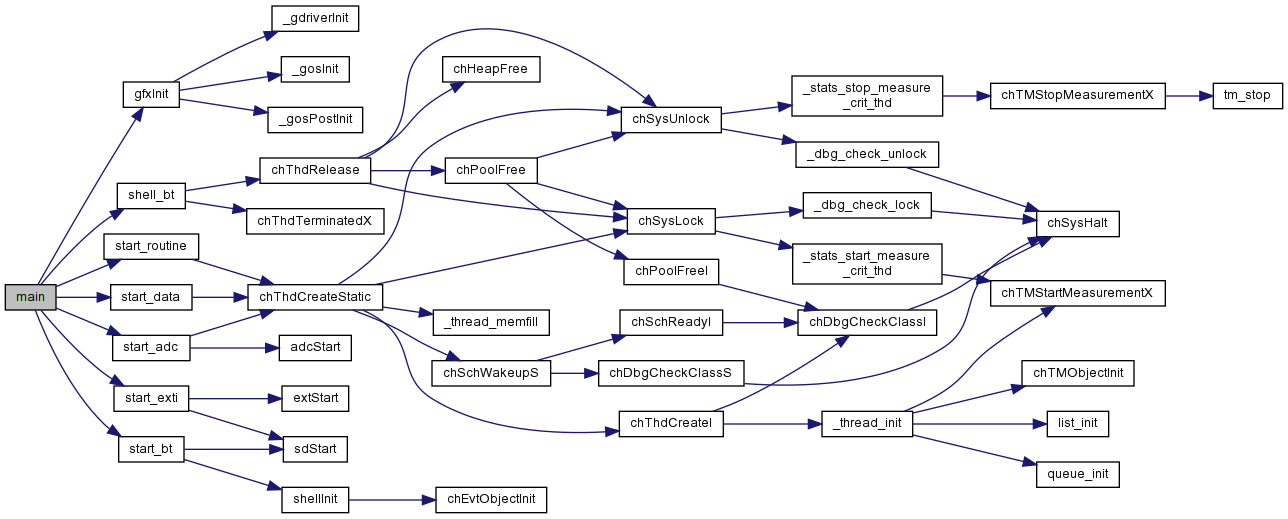
\includegraphics[width=\linewidth]{images/jw_ch_main}
		\caption{Firmware Main Modules}
	\end{figure}
		
	\subsection{Qt-based Desktop Interface}
	
	\subsection{Android Mobile Interface}
	
	\newpage
	\chapter{Prototype}
	
	\section{Introduction}
	
	\section{Hardware}
	
	\section{Hardware Bill of Material}
		
	\section{Software}
	
\end{document}